En esta sección se explican conceptualmente las decisiones de diseño de nuestro amplificador, se citan antecedentes investigados y se justifican cualitativamente algunas de las elecciones circuitales que se hicieron.
El diseño de un amplificador de tensión como un solo bloque que cumpla con las especificaciones, es una tarea de muy alta complejidad, pero se simplifica enormemente con el uso de técnicas de realimentación, comunes en la teoría de control, que se implementaron en este amplificador. 

\begin{figure}[H]
	\centering
	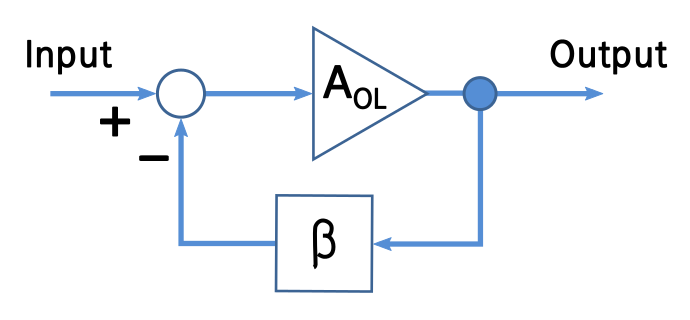
\includegraphics[width=0.5\textwidth]{img/realimentacion-negativa-bloque}
	\caption{Modelo general de realimentación negativa.}
	\label{fig:ampli_feedback}
\end{figure}


\subsection{Realimentación global}


Debido a la complejidad del circuito, cumplir con todas las especificaciones a lazo abierto es altamente complejo y requiere demasiada precisión en el cálculo y elección de componentes. Esto derivaría en un circuito altamente complejo y costoso. Es por este motivo que se emplea el realimentador. En esquema empleado se ve en la figura~\figref{fig:ampli_feedback_blocks}.

Dado que en un amplificador de audio se busca que la salida sea una versión de escalada de la señal de entrada, se busca tomar una muestra de la misma, y compararla con la señal de entrada. 

Como sabemos si se cumple que la ganancia de lazo cumple $a \cdot f \gg 1$, donde $a$ es la ganancia del amplificador a lazo abierto y $f$ la transferencia del realimentador, es esta última la que fija fija la ganancia a lazo cerrado, siendo la misma $A_{v} \simeq \frac{1}{f}$.

Una ventaja de esta técnica es que ayuda a que el amplificador se asemeje a un amplificador de tensión ideal, ya que aumenta la resistencia de entrada, mientras que disminuye la de salida. 

La realimantación es muy beneficiosa siempre que sea negativa. Dado que el sistema naturalmente introduce desfasajes, para ciertas frecuencias la realimentación puede pasar de ser negativa, a ser positiva (esto haría que las diferencias entre la señal de salida real y deseada se amplifiquen en lugar de reducirse) provocando que el circuito oscile a estas frecuencias. Para evitar que el circuito se vuelva inestable, es necesario que para las frecuencias donde se invierte la fase, el circuito pase de amplificar a atenuar, si esto no ocurre naturalmente, es necesario agregar componentes adicionales para compensar el circuito y evitar que se vuelva inestable.

Otro factor a tener en cuenta, es que puede darse la aparición de frecuencias en la salida del circuito fuera del rango de las que se presentan naturalmente en la entrada (en este caso $20 \si[per-mode=symbol]{\hertz} \longrightarrow 20 \si[per-mode=symbol]{\kilo\hertz}$ por tratarse de audio). También para eliminar estos inconvenientes es que el sistema debe ser compensado.

El uso de realimentación global permite mejorar notablemente casi todas las especificaciones del amplificador y simplificar su diseño (la estabilidad como se mencionó antes es una característica que puede empeorar, siendo el Slew-rate la otra que puede empeorar debido a la necesaria compensación). En este caso, como el objetivo es armar un amplificador de tensión, utilizamos un circuito realimentador Serie-Paralelo (muestrea tensión y suma tensión). El factor de realimentación queda definido por las especificaciones de sensibilidad y potencia RMS para una carga determinada.


\begin{figure}[H]
	\centering
	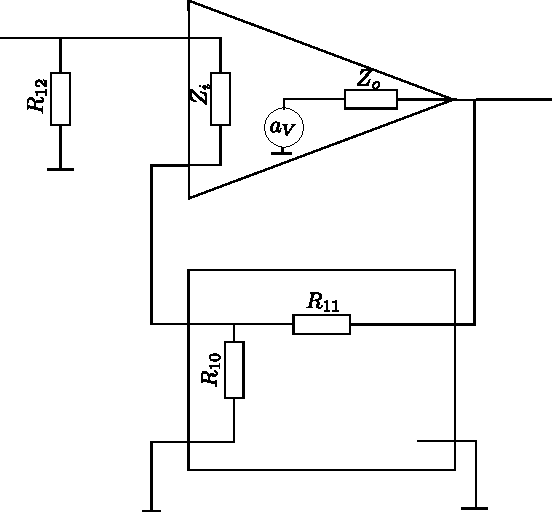
\includegraphics[width=0.5\textwidth]{img/realimentacion}
	\caption{Modelo amplificador-realimentación. El amplificador se encuentra realimentado con una topología serie-paralelo, muestreando tensión a la salida, y sumando tensión a la entrada, resultando un amplificador de ganancia de tensión estabilizado en tensión.}
	\label{fig:ampli_feedback_blocks}
\end{figure}


\subsection{Amplificador a lazo abierto}

Las etapas de un amplificador hacen referencia a su estructura a gran escala: el diagrama en bloques que modulariza los componentes y ayuda a diseñar, entender y evaluar su funcionamiento. La arquitectura de un amplificador típico consta, básicamente, de 3 etapas: una de entrada, diferencial, una intermedia, de ganancia de tensión, y una de salida, de ganancia de corriente o potencia (figura~\figref{fig:etapas}).

\begin{figure}[H]
	\centering
	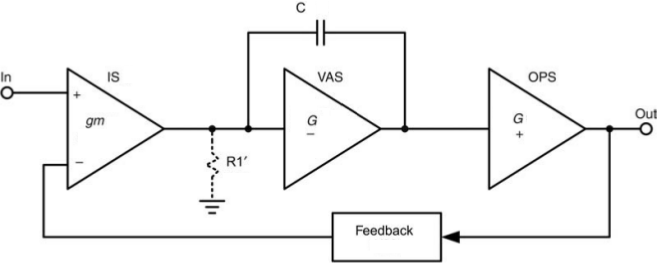
\includegraphics[width=0.6\textwidth]{img/etapas}
	\caption{Tres etapas de un amplificador típico, su realimentación y su capacitor de compensación (compensación por Miller). El esquema es genérico y no representa al amplificador diseñado.}
	\label{fig:etapas}
\end{figure}


Se han propuesto arquitecturas de dos etapas (como en \textbf{\quotemarks{\textit{Linsley-Hood, Simple Class-A amplifier , Wireless World [~April~1969~] p. 148}}} y en \textbf{\quotemarks{\textit{B. Olsson , Better audio from non-complements? Electronics World [~December~1994~] p. 988}}}) unificando la segunda y la tercera etapa. Sin embargo, dificulta el proceso de diseño sin grandes beneficios visibles, es poco común entre amplificadores comerciales, y suele ofrecer mala distorsión. También se han propuesto arquitecturas de cuatro etapas, como \textit{Lohstroh y Otala} en su paper \textbf{\quotemarks{\textit{An audio power amplifier for ultimate quality requirements}}}. Sin embargo, tampoco es muy usado en la industria, pues esta complejidad adicional no parece traer beneficios, al menos no en un amplificador discreto, es posible que no sea así en un diseño monolítico integrado.


El amplificador diseñado entonces tiene una \textbf{estructura típica de tres etapas}, aunque con la variante de ser completamente simétrico. La última etapa es la responsable de proveer la potencia y la que determina la eficiencia, tamaño y peso del amplificador; en particular, es la etapa que le da el nombre de amplificador, en nuestro caso, \textbf{Clase G}.


\subsection{Antecedentes}

El libro de Douglas-Self compila la vasta experiencia de un diseñador de amplificadores profesional. Es un libro de referencia y renombre en el mundo de los amplificadores de audio. Durante el diseño de este amplificador se tomó de referencia este libro para evaluar las opciones y sus ventajas y desventajas según la experiencia de la industria. El clase G de la figura~\figref{fig:ampli_DS} fue tomado directamente de su libro y estudiado. 

\clearpage

\begin{figure}[H]
	\centering
	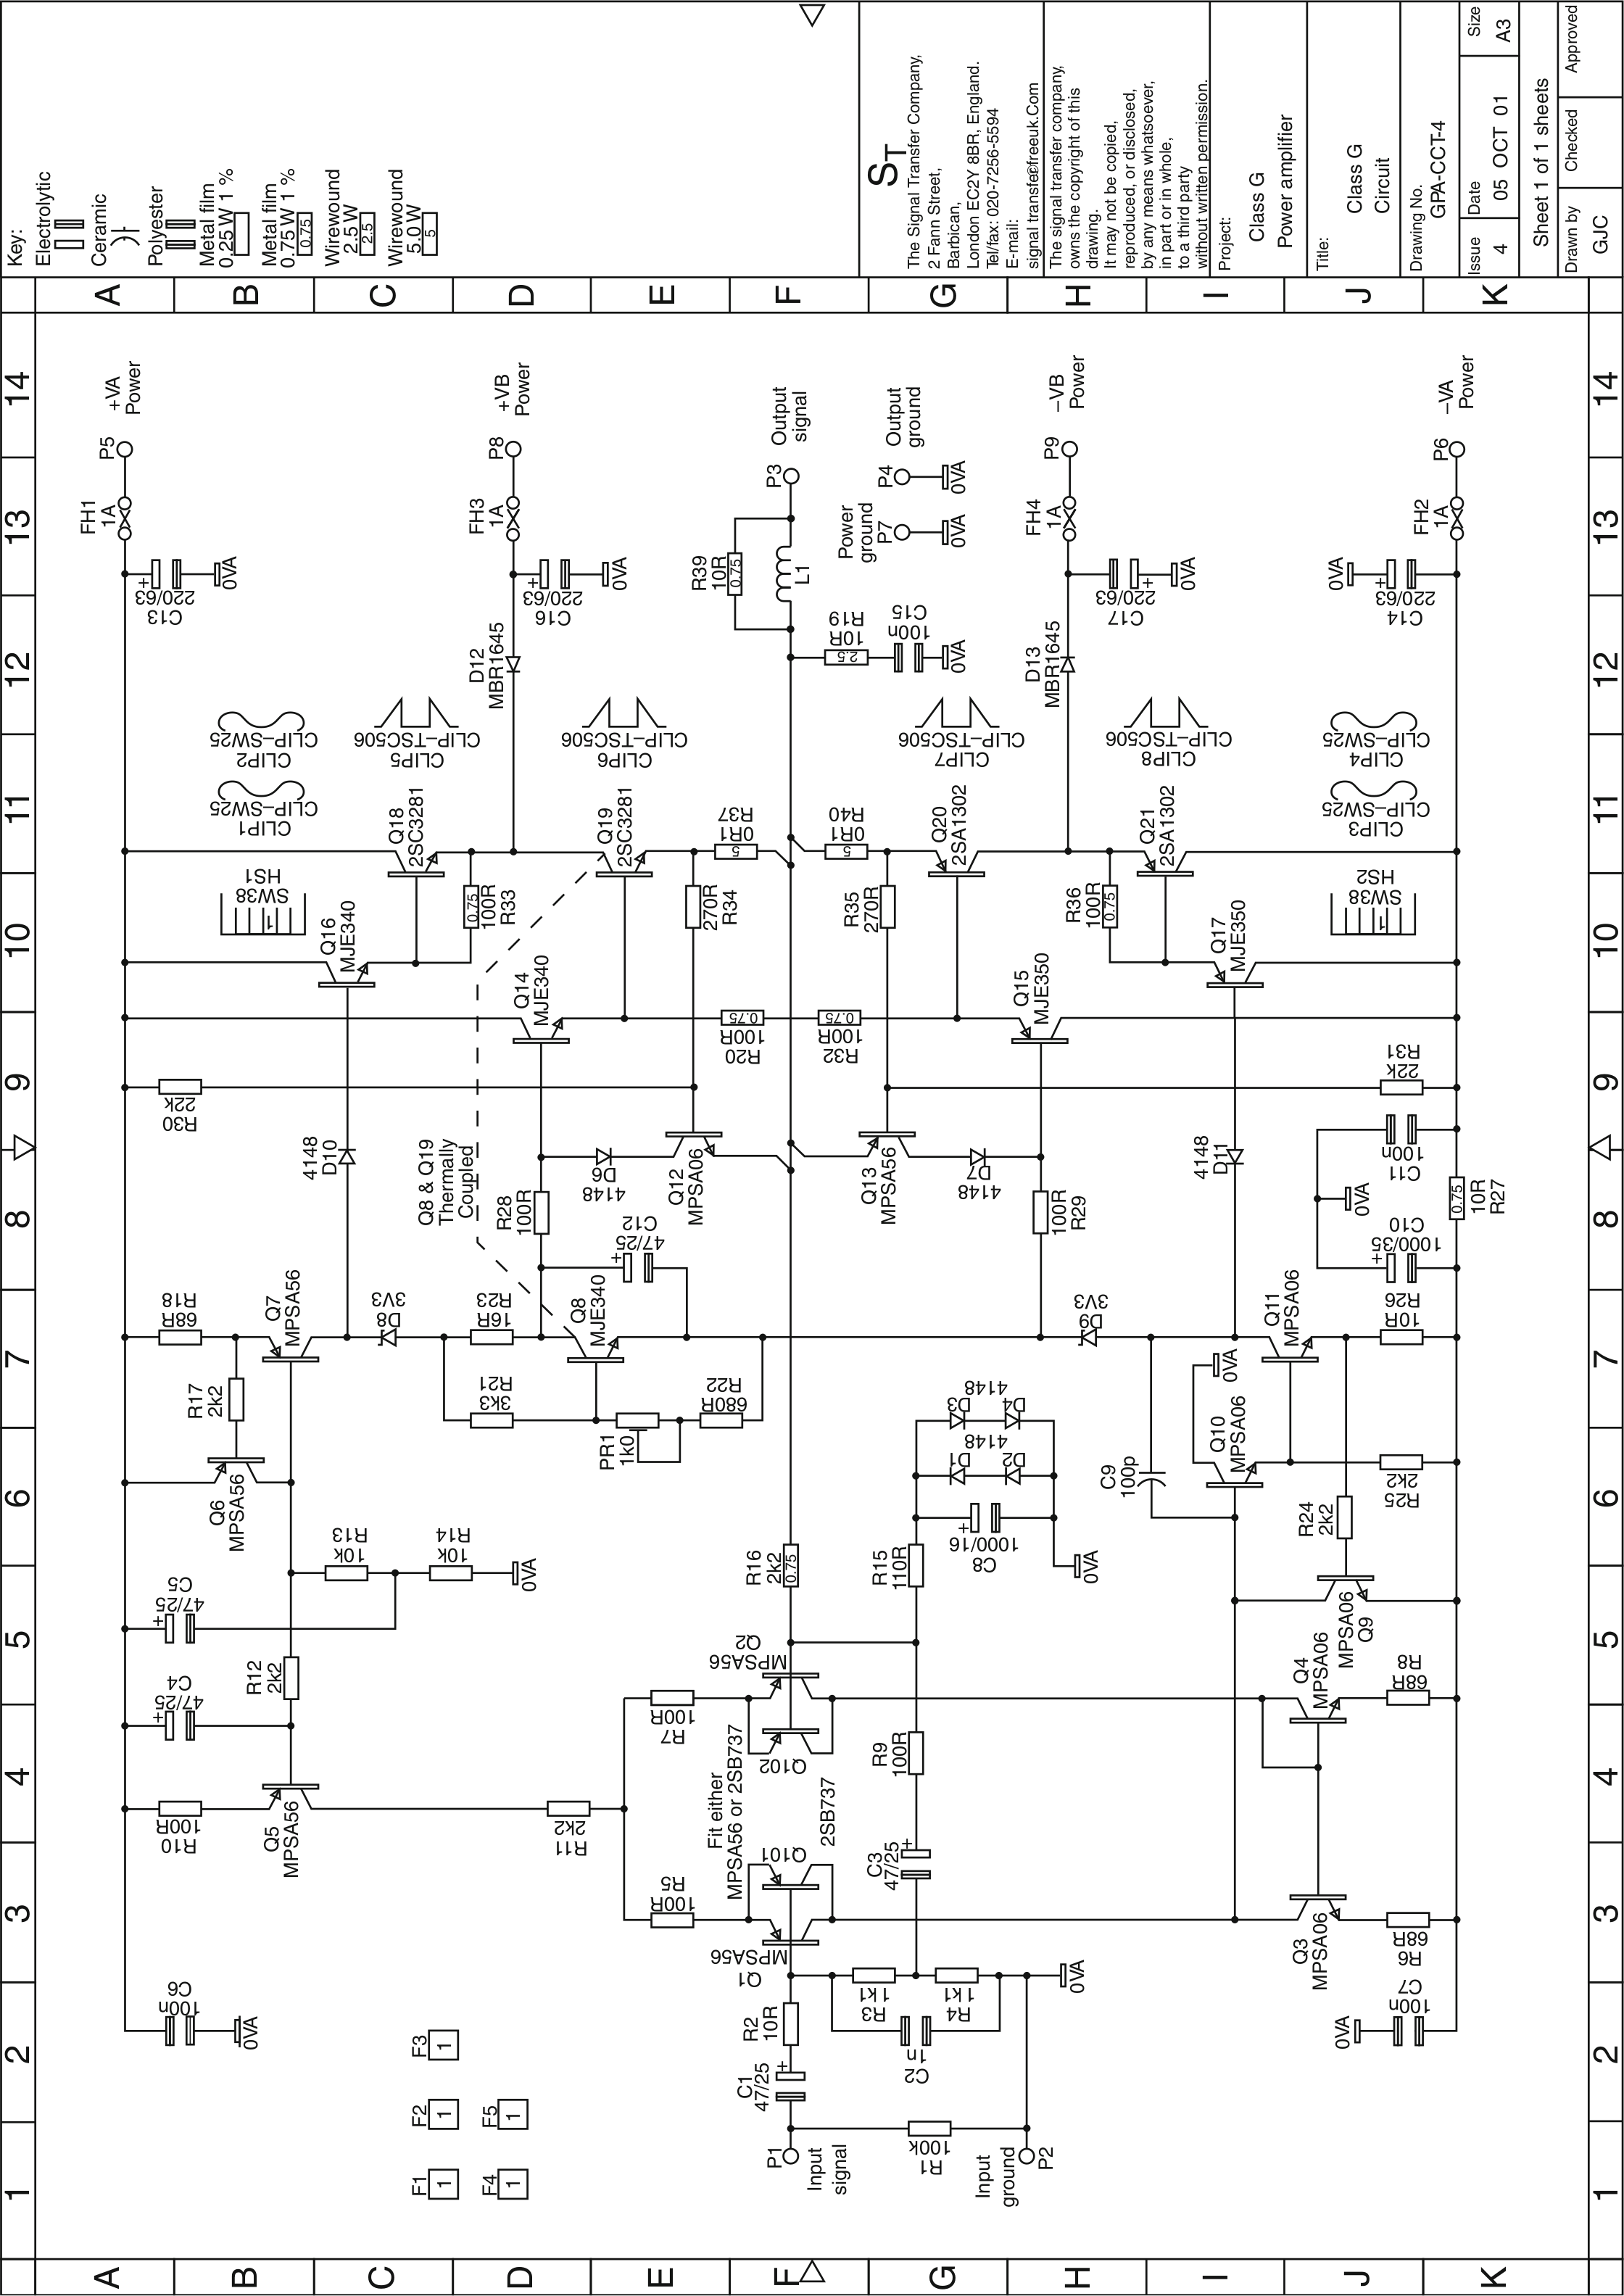
\includegraphics[width=0.86\textwidth]{img/clase_g_del_libro.png}
	\caption{Amplificador clase G, Douglas Self}
	\label{fig:ampli_DS}
\end{figure}


\clearpage

\subsection{Etapa de entrada}

En el esquema de tres etapas, la primera cumple la función de amplificar la diferencia entre sus dos entradas, rechazando las señales comunes. Esta capacidad de rechazo de las señales comunes es importante no sólo para implementar el modelo de realimentación planteado, sino para reducir el efecto de ruidos que afecten de forma igual a ambas entradas.
Sin embargo, esta simetría no es total: el comportamiento en un semiciclo difiere del comportamiento del semiciclo opuesto, por estas mismas alinealidades mencionadas. Se eligió entonces una topología de doble par diferencial. Es decir, propusimos agregar otro par, en paralelo, con componentes complementarios: donde originalmente usamos transistores \textbf{NPN}, colocamos \textbf{PNP}, y viceversa. De esta forma, la simetría cancela mas de las alinealidades y se reduce la distorsión aún más. Esto llevó a luego intentar mantener una simetría total en todo el circuito. 


Otra opción de diseño más, es la de la carga de los pares diferenciales. Estos pueden ser activas o pasivas. Por lo general, se elige una carga de tipo activa, como por ejemplo, una fuente de corriente espejo, porque da una menor distorsión, esto es típico en amplificadores operacionales, pero en nuestro caso, este diseño original fue descartado por consejo de los docentes, ya que, a pesar de tener un muy buen desempeño en las simulaciones, al ser implementado en la práctica presenta problemas de estabilidad en la polarización, de la charla con los docentes y posteriores simulaciones nos llevaron a elegir un amplificador tipo cascode, con una carga pasiva, porque necesitamos la caída en la carga para polarizar la etapa siguiente, donde explicaremos el motivo. 



Por último y no menos importante, es necesario determinar la forma de polarizar con corriente a los transistores de las ramas de los amplificadores diferenciales. Esto se hace mediante una fuente de corriente cuyo diseño puede tomar diversas formas: fuente espejo, semi-espejo, cascode, etc. Normalmente, se utiliza un transistor con una resistencia en serie en el emisor, y algún semiconductor en la base base, para fijar una tensión de polarización, mientras la resistencia antes mencionada determina la corriente de polarización que luego se dividirá a la mitad por las ramas del diferencial. La opción elegida hace uso de un par de diodos de señal (\textbf{1N4148}) que fijan la corriente del transistor en forma bastante independiente de la tensión de alimentación. Normalmente, estas fuentes, toman la referencia desde los rieles externos, porque son más estables que los internos, pero en este caso, al ser las tensiones de los rieles externos, muy elevados, preferimos utilizar unos reguladores lineales (\textbf{78L05} y \textbf{79L05}), para tomar de los rieles internos, y obtener $\pm 5 \si[per-mode=symbol]{\volt}$ de notable estabilidad, gracias al rechazo de ripple de $60 \si[per-mode=symbol]{\decibel}$ del regulador.


\subsection{Etapa de amplificación de tensión (VAS).}

Por lo general, la etapa de amplificación suele estar compuesta por un simple amplificador de configuración Emisor Común, entrando a la etapa de salida, por debajo del multiplicador de $V_{be}$, y polarizado por una fuente de corriente de colector. En este amplificador se optó por un diseño EF VAS: a este EC se le agrega una etapa colector común anterior, antes del amplificador. El seguidor cumple la función de para separar la etapa de entrada; esto mejora la distorsión. También se puede modificar para que la salida del VAS no sea por debajo del multiplicador de $V_{be}$, sino por el medio, para disminuir el offset a la salida, previo a la realimentación, y disminuir la distorsión. El inconveniente de este modo es que se necesitan dos fuentes de corriente más, ya que el modo anterior, aprovecha la fuente de polarización del EF VAS, para polarizar, también, el multiplicador de Vbe. En nuestro caso, con el cambio a 2 pares diferenciales, duplicamos la etapa EF VAS, complementariamente, y se conectan a la etapa de salida, por arriba y por abajo del multiplicador de $V_{be}$. Como en este caso, cada uno de los dos EF VAS hace de carga del otro, los EF VAS no tienen fuente de polarización, entonces se necesita que la etapa diferencial tenga una carga resistiva, para fijar la tensión de base de los EF VAS. Si hubieramos usado una carga tipo fuente espejo, habríamos logrado que la corriente en las ramas del par diferencial fuera igual, pero sin fijar ninguna tensión para polarizar la base de los EF VAS.

\subsection{Etapa de salida}
Esta etapa es la responsable de amplificar la potencia de la señal. Es decir, debe tener \textbf{alta eficiencia}, y \textbf{bajos niveles de distorsión}. Además, se busca \textbf{minimizar la impedancia de salida} para mantener un \textbf{alto factor de amortiguamiento} y evitar que el rebote acústico afecte el comportamiento del amplificador. 
La etapa de salida clase G está compuesta por dos o más niveles de alimentación que permiten incrementar la eficiencia del amplificador con respecto al clase B. Esto se logra ya que con tensiones bajas, se utilizará una fuente de tensión menor, preservando la máxima excursión posible sobre la carga que ofrece un clase B alimentado con la fuente de tensión mayor. Para señales con picos de baja amplitud en relación al valor medio, la mejora en la eficiencia es modesta. Sin embargo, en el caso en que la señal tenga picos considerables con respecto a su valor medio, la mejora es notable. Un punto importante, a la hora de diseñar una etapa de salida clase G, es la tensión de los rieles internos. Tomamos del libro de Douglas Self, los estudios realizados considerando los casos en los cuales la tensión de riel interno es de 30 y 60\% del externo, y se observó que los beneficios en cuanto a eficiencia, del segundo caso, son pocos. En cambio, en el caso de rieles internos de 30\% respecto de los externos, la eficiencia aumenta considerablemente. Otro detalle de diseño, es la del multiplicador de $V_{be}$ doble. El multiplicador de $V_{be}$ más simple, tiene un transistor, y 2 resistencias, con las que forma el salto de potencial necesario para eliminar el problema de cruce por 0 de la etapa de salida. En este caso, se usan 2 transistores complementarios, con la misma idea que el del doble par diferencial, para que el corrimiento de tensión del multiplicador de Vbe sea lo más lineal posible.

\subsubsection{Protección de cortocircuito}

%%\fxnote{Croto, en ubicación y contenido. tomado del Douglas, 5th ed, page 447 en adelante}

Opciones para protección de corriente

* Limitación de corriente simple (figura~\figref{fig:simple-current-limit})

Versión más básica. Cuando la corriente es tal que la caida en \texttt{Re1} supera, aproximadamente, los $0.7 \si[per-mode=symbol]{\volt}$, los transistores \texttt{TR1} y \texttt{RT4} conducen y desvían corriente de la base de \texttt{TR2}. Análogamente, para el semiciclo negativo, si la caída en \texttt{Re2} supera los $0.7 \si[per-mode=symbol]{\volt}$. Se muestrea corriente a través de \texttt{Re1} y \texttt{Re2}, que funcionan como resistencias de emisor y a la vez como sensores de corriente. Los valores de estas resistencias de emisor se deteminan por los requerimientos de eficiencia o estabilidad, por lo que el valor de corriente límite queda determinado por los divisores de tensión (\texttt{R1}-\texttt{R2} y el simétrico). 

%%\fxnote{Falta bastante. Falta que en gral con el simple hay líos que te hacen agregar otra protección en el VAS, aunque no la parece tener el clase G del Douglas. Hay otros tipos, y está el tema de que son sensibles a la temperatura y por eso pueden prenderse antes when hot y joder la distorsión. Hay que diseñarlos para todas las condiciones.}

\begin{figure}[H]
	\centering
	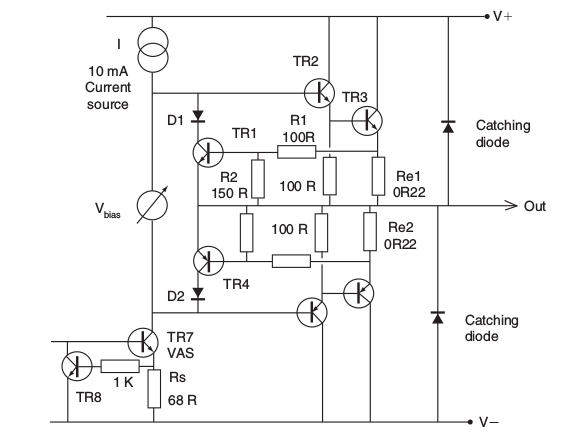
\includegraphics[width=0.6\textwidth]{img/simple-current-limit.png}
	\caption{Limitador de corriente simple}
	\label{fig:simple-current-limit}
\end{figure}



\subsection{Diagrama en bloques}

Finalmente en la figura~\figref{fig:ampli_bloques} se muestra un diagrama en bloques conceptual de nuestro circuito amplificador, mostrando en particular su estructura completamente simétrica.

\clearpage


\begin{figure}[H]
	\centering
	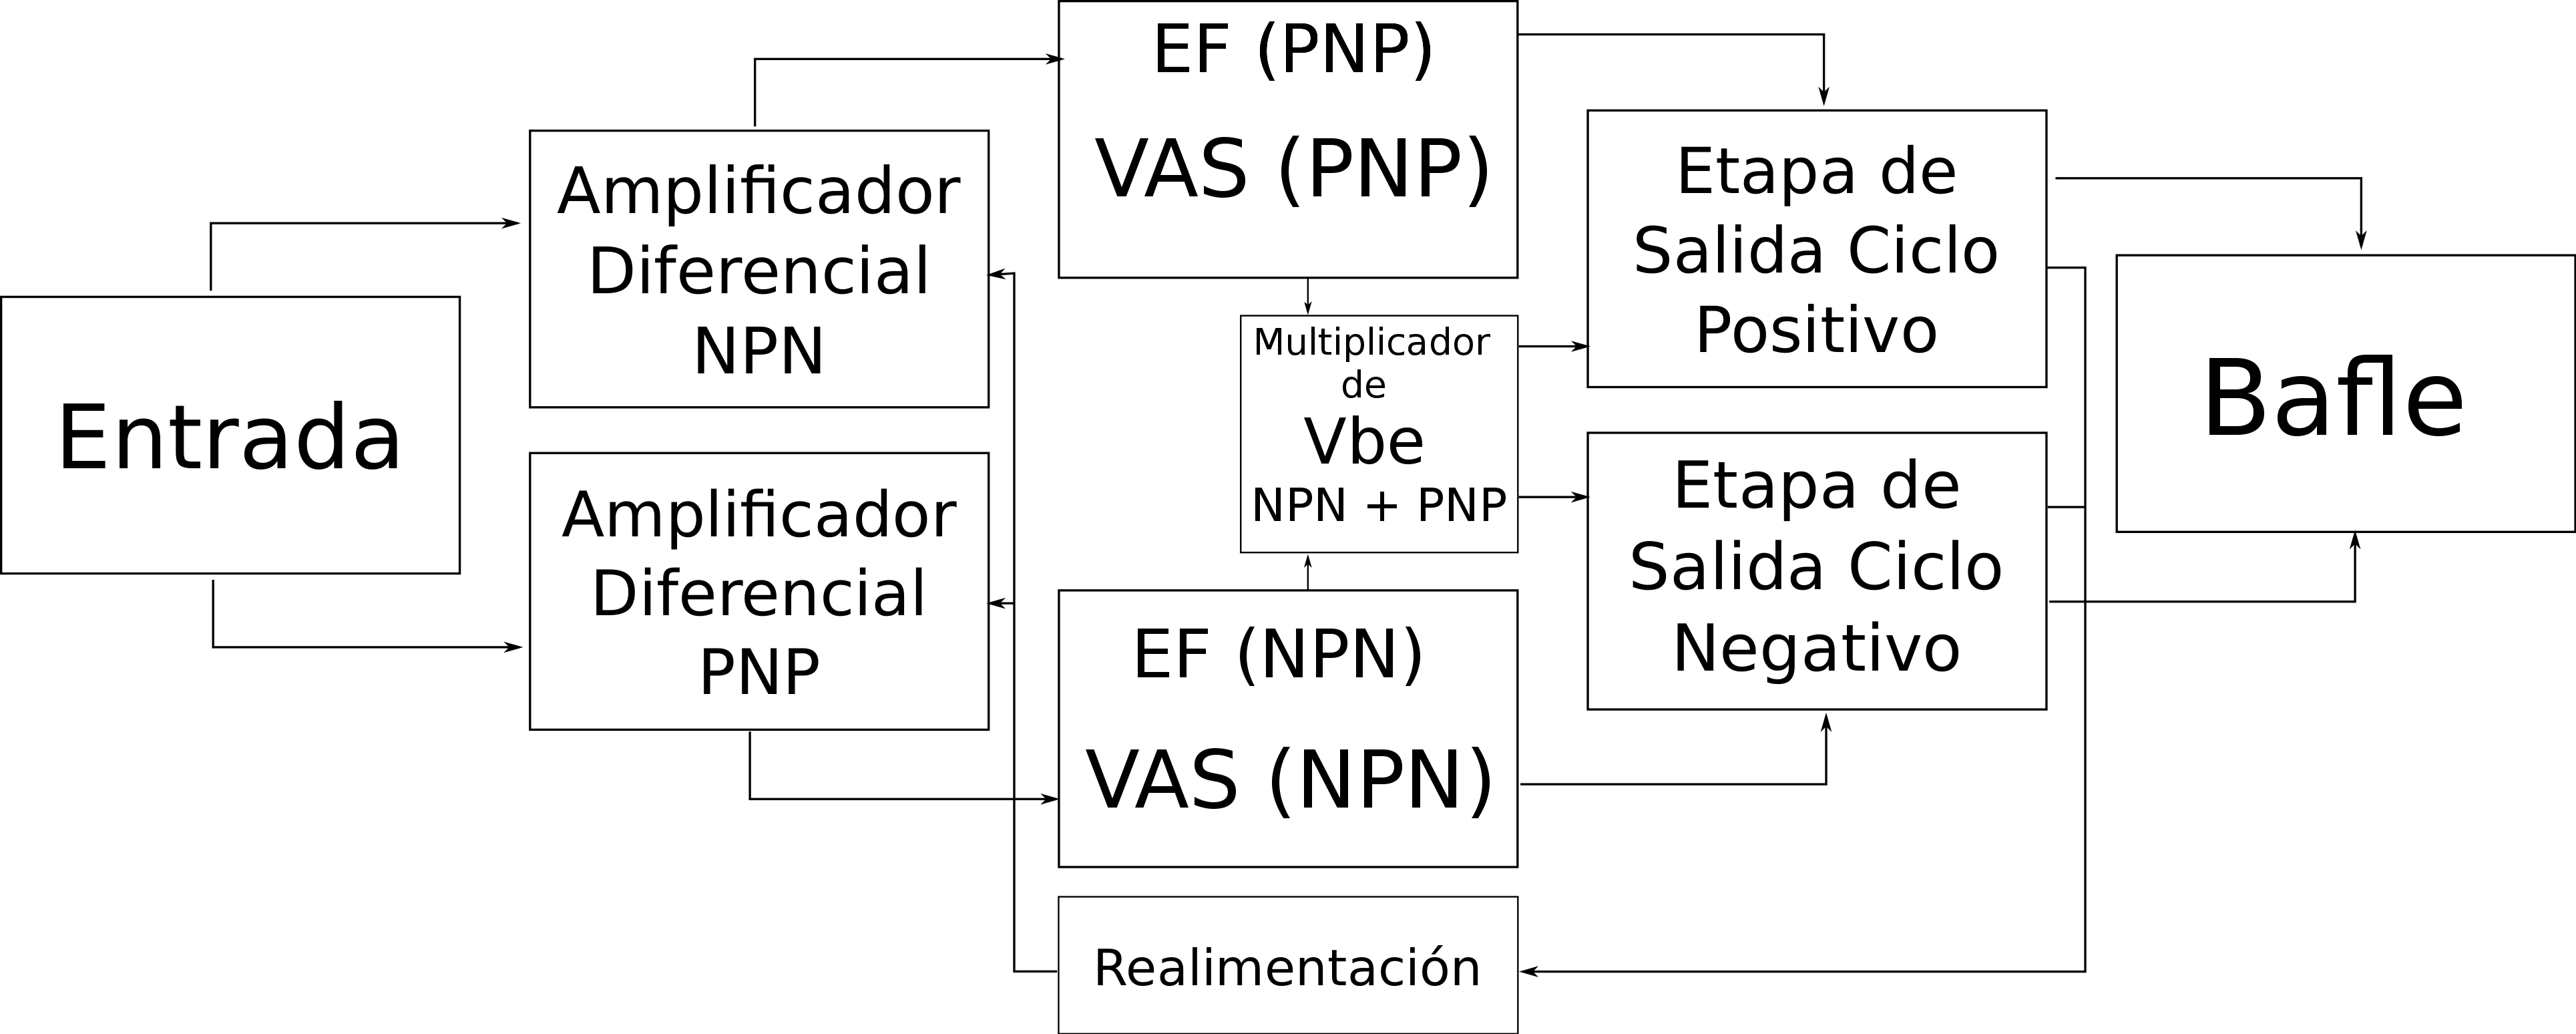
\includegraphics[width=0.9\paperwidth, angle=90]{img/bloques.png}
	\caption{Diagrama en bloques del amplificador clase G}
	\label{fig:ampli_bloques}
\end{figure}